\section{Background}
Metzler's and Westerhoff's model show that it is possible for endogenous business cycles to be induced through inventory cycles and the failure of firms to accurately predict future consumption. These models were designed to focus on the effects of firm expectations with Westerhoff's contribution consisting of introducing a heterogenous expectation rule that allows firms to switch behavior based on the state of the economy. Both of these models however simplify other aspects of the economy that feature more complex behavior in other business cycle models.

The inventory cycle model features 3 main factors of production: predicted consumption, investment, and inventory. Metzler and Westerhoff holds investment as an exogenously determined constant; however, this is both unrealistic and does not allow for long term endogenous growth. To incorporate a mechanism for endogenously adjusting investment, we take inspiration from the discrete time business cycle model described by T\"{o}nu Puu\autocite{Puu2003}. In order for investment to operate under Keynes' accelerator principle, capital stock must be in a proportion to the change in income, thus the investment level would be a function of the rate of change in income. 

A linear function for investment captures this premise; however, this leads to unrealistic behavior for higher magnitudes of income change. Suppose income dramatically increased; a linear function implies that a proportionally high level of investment can sustain this higher level of production when in reality other factors of production such as the land, labor, or technology available are the primary limiting factors. Of larger concern with a linear model though is if the economy encounters a sharp decrease in income. This induces a large, negative value for investment which implies that firms would actively destroy their machinery and other forms of capital stock in the event of an economic recession. This is obviously unrealistic and so John Hicks introduced a piecewise linear investment function such that at extreme levels of income change, investment will reach a predetermined maximal or minimal value. This piecewise function was then adapted to be differentiable over all points by Richard Goodwin by approximating the curve with a hyperbolic-tangent function\autocite{Puu2003}.

Puu approximates the hyperbolic-tangent function with its linear-cubic Taylor series expansion as this introduces a back-bending behavior into the curve. This allows the investment curve to capture not only firm behavior in the private sector but also implicitly include government spending and taxation. This follows from the now common policy for governments to engage in contracyclic behavior, increasing the quantity and size of spending projects and decreasing taxes when income is decreasing. Likewise, when the economy is performing well, the government cuts back on spending projects intended to stimulate the economy while also increasing taxes in order to take advantage of the overheating economy. 

The problem with the cubic function is that it leads to unbounded behavior in the extremes, much like the linear function. Puu resolves this by ensuring that income growth is bounded by [-1, 1]; this is not the case for our model however. We instead want a function that features similar curvature and behavior as the cubic function but flattens when income change is of significant magnitude. This can be accomplished with the following function:

\begin{equation}
    I_t = \frac{\frac{Y_{t-1}-Y_{t-2}}{v}}{(\frac{Y_{t-1}-Y_{t-2}}{v})^4+q}	
\end{equation}

The behavior of this function qualitatively resembles that of the linear-cubic function described in by Puu when $v,q>0$ and ; however, $\lim_{(Y_{t-1}-Y_{t-2})\to\infty}I_t=0$. This function is at its absolute maximum and minimum when:
\begin{equation*}
    Y_{t-1}-Y_{t-2}=\pm\frac{q^{1/4}v}{3^{1/4}}
\end{equation*}
Thus giving a maximal or minimal investment of:
\begin{equation*}
    I_t=\frac{3^{3/4}}{4q^{3/4}}
\end{equation*}
Intuitively, larger values of $v$ make the function "wider", increasing the range over $Y_{t-1}-Y_{t-2}$ where $I_t$ is not effectively 0. Smaller values of $q$ increases the magnitude of the maximum and minimum of the function, effectively making it taller. $v$ and $q$ cannot be directly attributed to any direct economic phenomena; however, their effect on the function can be interpreted analogously to the properties of the linear-cubic function. The "height" of the function determines the potential magnitude of investment and the "width" determines the rate at which investment, both private and public, react to changes in income.

Metzler describes the existence of two important lags in the study of Keynesian models. The Robertson lag is characterized by making current consumption a function of past income, i.e. consumption behavior lags behind current income. The Lundberg lag however concerns a discrepancy between the income level and the production decision of firms \autocite{Metzler1941} . These lags are named after the two economists D. H. Robertson and Erik Lundberg who developed models that contained only their eponymous lag type. Although both lags are likely to exist in reality, most models only incorporate one lag due to the increased complexity associated with it. Metzler and Westerhoff make use of a Lundberg lag by making income a function of the predicted level of consumption as opposed to actual consumption. T\"{o}nu Puu's model makes use of a Robertson in order to induce endogenous business cycles. Metzler himself does not claim that the Lundberg sequence is any more realistic than the Robertson sequence. Whichever lag has a longer time-period can be treated as of being greater importance but Metzler actually proposes a variety of scenarios that present contradicting conclusions. Suppose that decided their behavior on a quarterly basis but consumers altered their spending behavior with every paycheck, then it is no longer unrealistic to treat the Robertson lag as being of 0 length, i.e. nonexistent. If consumers revise their spending behavior every 6 months to a year, then it would actually be more realistic to include a non-zero Robertson lag while minimizing the Lundberg lag. 

For the purposes of this model, we will include a non-zero Lundberg and Robertson lag. The consumption function is treated exactly as presented in Puu:
\begin{equation}
    C_t=(1-s)Y_{t-1}+sY_{t-2}
\end{equation}
This function incorporates a 1-period Lundberg lag where $s\in[0,1]$ is the marginal propensity to save. This function also contains a 2-period delayed consumption due to the marginal propensity to save, thus all income made in some period $t$ can be though of as being eventually spent in the period $t+1$ and $t+2$. Although intuitive, this explanation is not wholly accurate as the Lundberg lag does not imply saving of income to spend in the next period but rather that spending behavior is influenced only on the information of lagged income level. The choice of $s$ dictates the relative importance of lagged income, a higher marginal propensity to save reduces the impact of income made in the previous time period but increases the effective impact of the income made two time periods ago.  

As the economy is also making use of a Robertson lag, income is not directly a function of consumption as may be seen in other models. Rather, income is viewed from a production standpoint. This is achieved by explicitly defining a predicted level of consumption. Westerhoff and Metzler use an equation similar to the form:

\begin{equation*} 
    U_t=C_{t-1}+\eta(C_{t-1}-C_{t-2})
\end{equation*}
However, this assumes that firms have no way to adapt their coefficient of expectation $\eta$. 

A new predictive mechanism requires that firms have bounded rationality. If firms possessed perfect rationality, then they would be able to perfectly predict consumption levels as consumption is based on lagged income, thus if we wish to maintain our Robertson lag, firms must still have bounded rationality. Another mechanism that firms can use that maintains better "memory" is that of an average. 
\begin{equation}\label{predict}
    U_t = \frac{C_{t-1}+C_{t-2}+C_{t-3}}{3}
\end{equation}
This formulation is an average of the consumption levels of the past 3 time periods. The choice of three time periods is relatively arbitrary and higher order difference equations of the same form can be used; however these higher order formulations can result in a less mathematically tractable model.

Inventory production proceeds as seen in Chapter 2 with firms producing $S_t$ explicitly to maintain Inventory at optimal levels:
\begin{equation}
    S_t = k U_t-Q_{t-1}
\end{equation}
where $Q_t$ is the level of inventory maintained at the end of time $t$ and $k\in[0,1]$. This can be solved for as the sum of the previous inventory level, production intended for inventory, and the difference between production intended for consumption and the actual consumption level:
\begin{equation}
    Q_t=Q_{t-1}+S_t+(U_t-C_t)
\end{equation}

Income level, or output, can thus be written as a sum of production:
\begin{equation}\label{eq:Income}
    Y_t=I_t+S_t+U_t
\end{equation}
However, as income has the capability of sustained growth under this model, it is preferable to analyze the rate of change of income in this model. In Appendix A, we show that the growth rate of the economy can be interpreted as a single variable, 6th order difference equation on $\dot Y$:
\begin{equation}
\begin{split}
    \dot Y_{t}& = \frac{\frac{\dot Y_{t-1}}{v}}{\left(\frac{\dot Y_{t-1}}{v}\right)^4+q}-\frac{\frac{\dot Y_{t-2}}{v}}{\left(\frac{\dot Y_{t-2}}{v}\right)^4+q} + \\
    & (1+k)\frac{(1-s)(\dot Y_{t-2}+\dot Y_{t-3}+\dot Y_{t-4})+s(\dot Y_{t-3}+\dot Y_{t-4}+\dot Y_{t-5})}{3} -\\
    &\left[(k+1)\frac{(1-s)(\dot Y_{t-3}+\dot Y_{t-4}+\dot Y_{t-5})+s(\dot Y_{t-4}+\dot Y_{t-5}+\dot Y_{t-6})}{3}\right.\\
    &\left.-(1-s)\dot Y_{t-2}-s\dot Y_{t-3}\right]
\end{split}
\end{equation}

\section{Growth Dynamics}
The long run dynamics of the model are highly dependent on the choice of initial conditions. Simulation of the model require a choice of 6 initial values of income change in addition to the parameter choice. If the 6 initial values are equivalent, all future iterations of the mapping are equal to this choice and the model remains in a stable steady state. It both more interesting and realistic then to consider cases where there is variation in initial income growth.
\begin{figure}[ht]
    \centering
    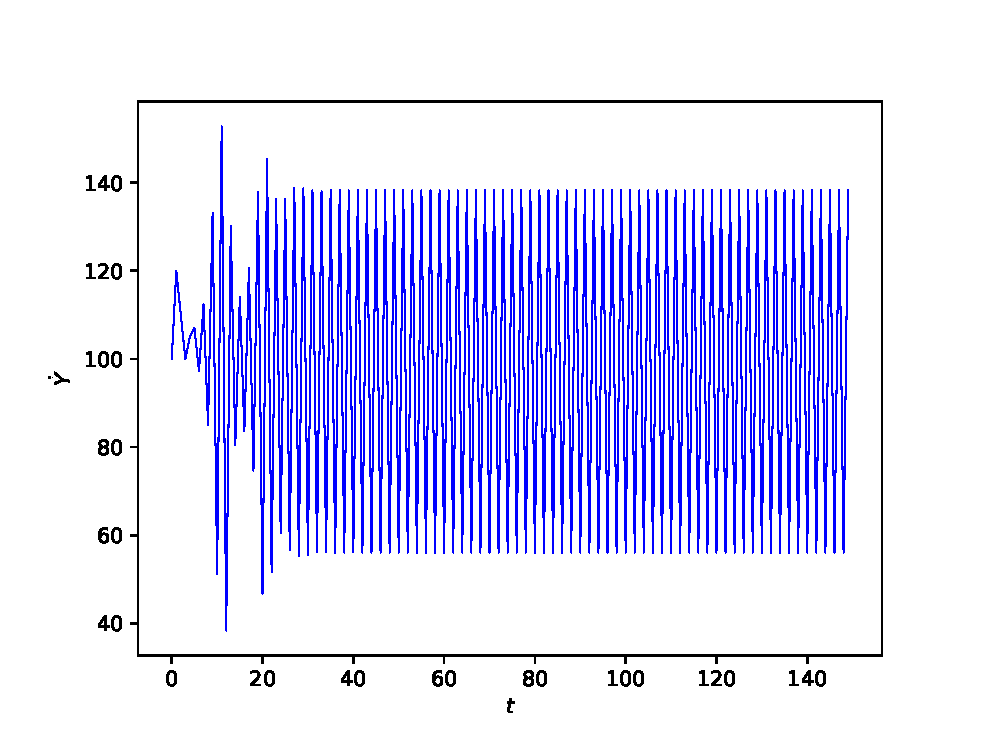
\includegraphics[height=0.4\textheight]{./metzlerian_growth/timeseries1.eps}
    \caption{Timeseries plot of income growth rate over 150 iterations. $s=0.6,\ k=0.3,\ v=500,\ q=0.001$. Initial values of $\dot Y$ are: 100, 120, 110, 100, 105, 107}
    \label{growth_timeseries1}
\end{figure}
Figure \ref{growth_timeseries1} displays a possible trajectory of income growth. Under the parameters listed, the trajectory clearly behaves in a stable, cyclic manner within 40 iterations. 

There do not exist techniques to solve generalized 6th order difference equations; however it is possible to computationally solve for the long run dynamics of the system.
\begin{figure}
    \centering
    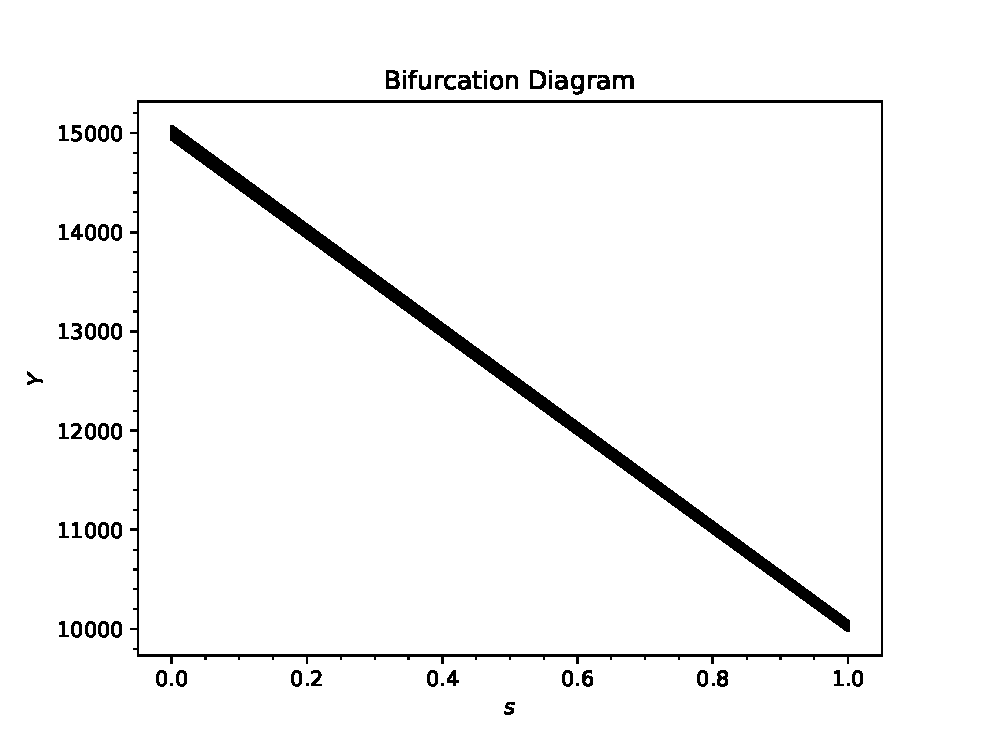
\includegraphics[height=0.4\textheight]{./metzlerian_growth/sbifurcation}
    \caption{Bifurcation diagram varying $s$ between 0.1 and 0.9. Initial conditions and other parameters are held constant as described in Figure \ref{growth_timeseries1}.}
    \label{metzlerian_growth-sbifurcation}
\end{figure}

The bifurcation diagram displayed in Figure \ref{metzlerian_growth-sbifurcation} displays the long-run behavior of the model as $s$ is varied. The methodology of the computational analysis and results are displayed in detail in Section \ref{bifurcation_analyzer} and Section \ref{bifurcation_analysis}, respectively. Long-run values are rounded to their nearest whole number for the purposes of this computational analysis although it is possible to account for higher levels of numerical precision using the analyzer. A bifurcation point exists at $s=0.65$ and $s=0.53$, the mapping is a stable 2 cycle when $s$ is between these two values. This implies the presence of a stable business cycle when the marginal propensity to save is moderately high; however, the behavior appears chaotic when the marginal propensity to save approaches either extreme. 

\begin{figure}
    \centering
    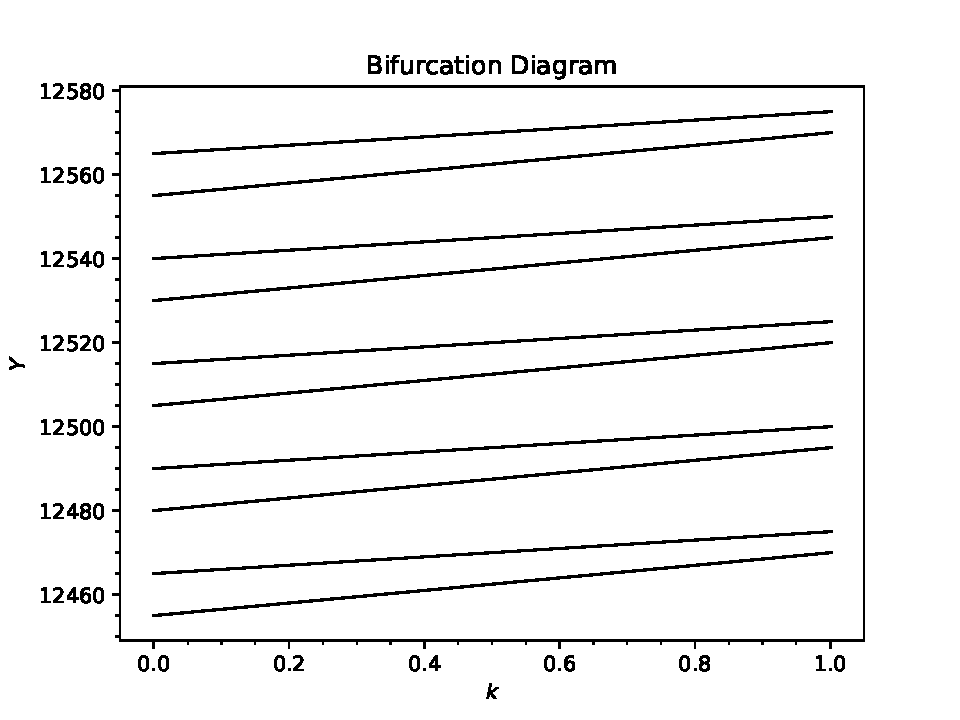
\includegraphics[height=0.4\textheight]{./metzlerian_growth/kbifurcation}
    \caption{Bifurcation diagram varying $k$ between 0.1 and 0.9. Initial conditions and other parameters are held constant as described in Figure \ref{growth_timeseries1}.}
    \label{metzlerian_growth-kbifurcation}
\end{figure}

The bifurcation diagram varying $k$ seen in Figure \ref{metzlerian_growth-kbifurcation} qualitatively appears much simpler than Figure \ref{metzlerian_growth-sbifurcation}. This diagram displays a bifurcation point when $k\approx 0.84837$. The model displays stable 2-cycle behavior until this point although the system continues to display windows of ordered cycles. It thus appears that although increasing the desired proportional level of inventory does increase the long-run level of cyclic growth, it does not affect the topology until $k$ is unrealistically large. 

\begin{figure}
    \centering
    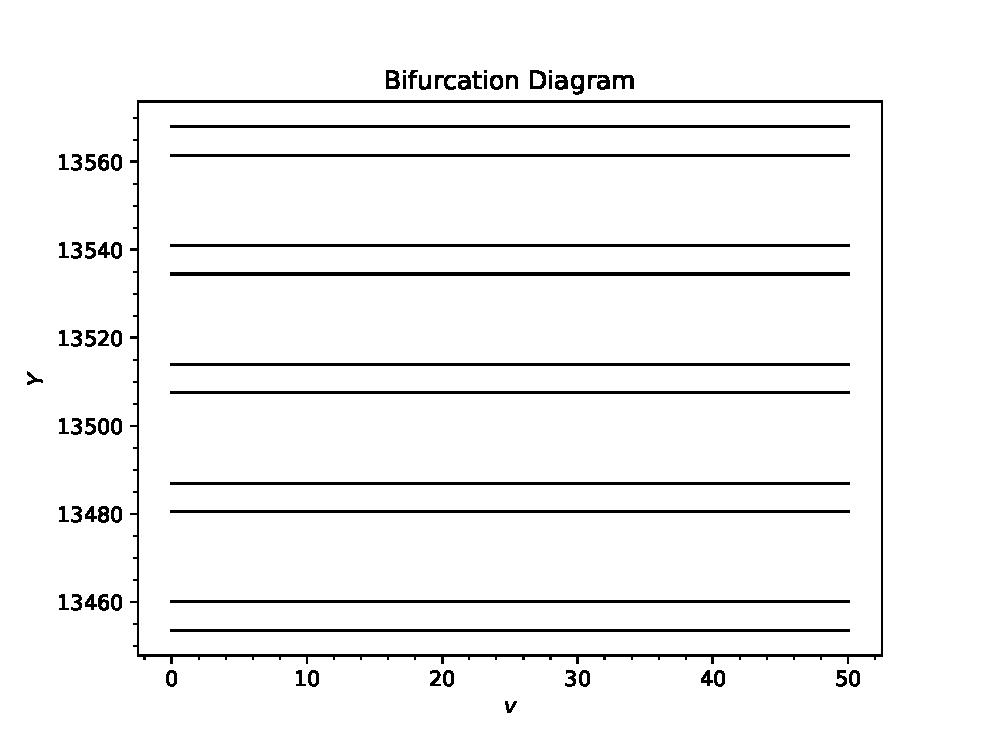
\includegraphics[height=0.4\textheight]{./metzlerian_growth/vbifurcation}
    \caption{Bifurcation diagram varying $v$ between 1 and 2000. Initial conditions and other parameters are held constant as described in Figure \ref{growth_timeseries1}.}
    \label{metzlerian_growth-vbifurcation}
\end{figure}
\begin{figure}
    \centering
    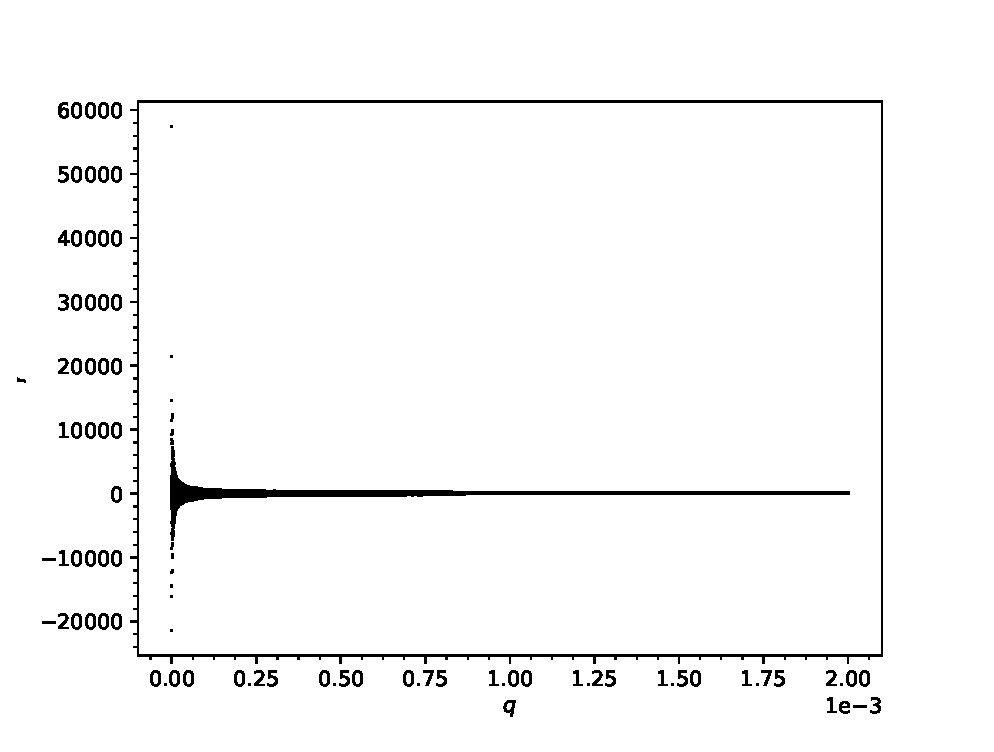
\includegraphics[height=0.4\textheight]{./metzlerian_growth/qbifurcation}
    \caption{Bifurcation diagram varying $q$ between 0 and 0.0001. Initial conditions and other parameters are held constant as described in Figure \ref{growth_timeseries1}.}
    \label{metzlerian_growth-qbifurcation}
\end{figure}

Figure \ref{metzlerian_growth-vbifurcation} exhibits stable, fixed growth when $v\in[1,297.338)\cup(617.104, 2000]$ which is the upper bound of what was computationally determined. The model also displays a stable 2-cycle when $v\in(472.173, 589.757)$. Likewise, Figure \ref{metzlerian_growth-qbifurcation} has a bifurcation point at $q\approx0.0015997$ and $q\approx0.0015976$ which mark transitions from a stable, fixed point to a 2-period cycle to a 3-period cycle (more bifurcation points exist within the diagram and are more easily viewed by narrowing the parameter variation range). As stated previously, $v$ and $q$ individually lack an economic interpretation, but together they approximate the dynamics of a linear-cubic investment curve while incorporating bounded, asymptotic behavior. 

These bifurcation diagrams do not tell the complete story of this model however for any given set of parameters. As stated previously, 
\subsection{Chaotic Behavior in Growth}
Bifurcation analysis of this type allows us to determine the presence and location of bifurcation points separating arbitrary period cycles. However, this is insufficient to determining if varying the parameters of the model result in chaotic behavior and where exactly this transition occurs. The existence of chaos lends credence to the assumption of bounded rationality assigned to firms. If the model always features stable cycles, then it would only be logical that firms would eventually be able to adapt their predictive mechanism to predict this ordered behavior. The effect this shift in expectation rule would have on future dynamics is beyond the scope of this paper; however, the presence of chaos means the model is sufficiently sensitive to initial conditions that firms would not be able to accurately determine the future state of the market as under a chaotic system, knowing the approximate current state of the economy does not inform firms of the approximate future state of the economy. 

We begin by rewriting the model as a 1st-order difference equation with 6 variables. This can be done by creating and defining the variables $\dot Y_{t-1}=\dot A_t$, $\dot A_{t-1}=\dot B_{t}$, $\dot B_{t-1}=\dot C_{t}$, $\dot C_{t-1}=\dot D_{t}$, and $\dot D_{t-1}=\dot G_{t}$. This allows us to define an equivalent model:
\begin{align*}
    \dot Y_t = f(\dot Y_{t-1}, \dot A_{t-1}, \dot B_{t-1}, \dot C_{t-1}, \dot D_{t-1}, \dot G_{t-1})\\
    \dot A_t = g(\dot Y_{t-1}, \dot A_{t-1}, \dot B_{t-1}, \dot C_{t-1}, \dot D_{t-1}, \dot G_{t-1})\\
    \dot B_t = h(\dot Y_{t-1}, \dot A_{t-1}, \dot B_{t-1}, \dot C_{t-1}, \dot D_{t-1}, \dot G_{t-1})\\
    \dot C_t = j(\dot Y_{t-1}, \dot A_{t-1}, \dot B_{t-1}, \dot C_{t-1}, \dot D_{t-1}, \dot G_{t-1})\\
    \dot D_t = l(\dot Y_{t-1}, \dot A_{t-1}, \dot B_{t-1}, \dot C_{t-1}, \dot D_{t-1}, \dot G_{t-1})\\
    \dot G_t = m(\dot Y_{t-1}, \dot A_{t-1}, \dot B_{t-1}, \dot C_{t-1}, \dot D_{t-1}, \dot G_{t-1})
\end{align*}
The Jacobian matrix of this system of equations is:
\begin{equation*}
J = \begin{bmatrix}
    \frac{\partial f}{\partial \dot Y_{t-1}} & \frac{\partial f}{\partial \dot A_{t-1}} & \frac{\partial f}{\partial \dot B_{t-1}} & \frac{\partial f}{\partial \dot C_{t-1}} & \frac{\partial f}{\partial \dot D_{t-1}} & \frac{\ f}{\partial \dot G_{t-1}}\\
    \frac{\partial g}{\partial \dot Y_{t-1}} & \frac{\partial g}{\partial \dot A_{t-1}} & \frac{\partial g}{\partial \dot B_{t-1}} & \frac{\partial g}{\partial \dot C_{t-1}} & \frac{\partial g}{\partial \dot D_{t-1}} & \frac{\ f}{\partial \dot G_{t-1}}\\
    \frac{\partial h}{\partial \dot Y_{t-1}} & \frac{\partial h}{\partial \dot A_{t-1}} & \frac{\partial h}{\partial \dot B_{t-1}} & \frac{\partial h}{\partial \dot C_{t-1}} & \frac{\partial h}{\partial \dot D_{t-1}} & \frac{\ f}{\partial \dot G_{t-1}}\\
    \frac{\partial j}{\partial \dot Y_{t-1}} & \frac{\partial j}{\partial \dot A_{t-1}} & \frac{\partial j}{\partial \dot B_{t-1}} & \frac{\partial j}{\partial \dot C_{t-1}} & \frac{\partial j}{\partial \dot D_{t-1}} & \frac{\ f}{\partial \dot G_{t-1}}\\
    \frac{\partial l}{\partial \dot Y_{t-1}} & \frac{\partial l}{\partial \dot A_{t-1}} & \frac{\partial l}{\partial \dot B_{t-1}} & \frac{\partial l}{\partial \dot C_{t-1}} & \frac{\partial l}{\partial \dot D_{t-1}} & \frac{\ f}{\partial \dot G_{t-1}}\\
    \frac{\partial m}{\partial \dot Y_{t-1}} & \frac{\partial m}{\partial \dot A_{t-1}} & \frac{\partial m}{\partial \dot B_{t-1}} & \frac{\partial m}{\partial \dot C_{t-1}} & \frac{\partial m}{\partial \dot D_{t-1}} & \frac{\ f}{\partial \dot G_{t-1}}
\end{bmatrix}
\end{equation*}
\begin{equation}
J=
\begin{bmatrix}\small
    \frac{\partial f}{\partial Y_{t-1}} & \frac{\partial f}{\partial A_{t-1}} & s+\frac{k+1}{3}s & 0 & \frac{(k+1)(s-1)}{3} & -\frac{(k+1)s}{3}\\
    1 & 0 & 0 & 0 & 0 & 0\\
    0 & 1 & 0 & 0 & 0 & 0\\
    0 & 0 & 1 & 0 & 0 & 0\\
    0 & 0 & 0 & 1 & 0 & 0\\
    0 & 0 & 0 & 0 & 1 & 0
\end{bmatrix}
\end{equation}
where 
\begin{align*}
    \frac{\partial f}{\partial Y_{t-1}}&= \frac{1}{v\left(q+\frac{Y_{t-1}^4}{v^4}\right)}-\frac{4Y_{t-1}^4}{v^5\left(q+\frac{Y_{t-1}^4}{v^4}\right)}\\
    \frac{\partial f}{\partial A_{t-1}}&=1+\frac{1}{3}(k+1)(1-s)-s+\frac{4A_{t-1}^4}{v^5\left(q+\frac{A_{t-1}^4}{v^4}\right)^2}-\frac{1}{v\left(q+\frac{A_{t-1}^4}{v^4}\right)}
\end{align*}











